\chapter{A Method for Tracking Centre of Mass Displacement During Non-Seated Cycling Using an Inertial Sensor}
\label{Chap:B}	%CREATE YOUR OWN LABEL.
\pagestyle{headings}

\section{Abstract}
Instantaneous crank power does not equal total joint power if a rider's centre of mass (CoM) gains and loses mechanical energy. Thus, estimating CoM motion and the associated energy changes can provide valuable information about cycling performance. To date, an accurate and precise method for tracking CoM motion during outdoor cycling has not been validated. \textbf{Purpose:} To assess the suitability of an inertial measurement unit (IMU) for tracking CoM motion during non-seated cycling by comparing vertical displacement derived from an inertial sensor mounted to the lower back of the rider to an attached marker cluster and to a kinematic estimate of vertical CoM displacement from a full-body musculoskeletal model (Model). \textbf{Methods:} IMU and motion capture data were collected synchronously for 10 seconds while participants (n=7) cycled on an ergometer in a non-seated posture at three power outputs and two cadences. A limits of agreement analysis, corrected for repeated measures, was performed on the range of vertical displacement between the IMU and the two other measures. A total of 303 crank cycles were analysed. \textbf{Results:} The IMU measured vertical displacement of the marker cluster with high accuracy (1.6 mm) and precision (3.5 mm) but substantially overestimated the kinematic estimate of rider CoM displacement. \textbf{Conclusion:} We interpret these findings as evidence that a single IMU placed on the lower back is unsuitable for tracking rider CoM displacement during non-seated cycling if the linearly increasing overestimation is unaccounted for.

\section{Introduction}
During non-seated cycling, tracking a rider's centre of mass (CoM) position can provide valuable information regarding rider and bicycle performance. At each instant during the crank cycle, the power output a rider generates is not equal to their total joint power if their CoM loses and gains mechanical energy \autocite{VanIngenSchenau1990b}. Previous research on non-seated cycling shows that a rider's CoM can gain and lose mechanical energy at rates of up to 4.5 W$\cdot$kg$^{-1}$ \autocite{Wilkinson2020b}, which has a significant effect on peak force and power production within each crank cycle. Thus, combining crank power measurements with an estimate of CoM energy changes could provide valuable insights into how riders maximise gross efficiency and maximal power output.

Estimating a rider's CoM position while cycling on an ergometer, treadmill, or over-ground can be done using an optical motion capture system. However, there are limitations to each of these experimental setups. Although ergometers allow multiple cycles to be collected per trial, they constrain the lateral dynamics of the bicycle, which changes the preferred movement pattern of the rider and may affect performance (See Chapter \ref{Chap:5}). Treadmills can provide a solution to ecological validity, but performing maximal sprinting is problematic due to the danger of matching the belt velocity to the rapid acceleration and high velocity of the bicycle wheels. Over-ground cycling can be captured, but the calibrated volume of the camera system will limit the number of cycles that can be collected. Thus, a method for tracking a rider's CoM motion when motion capture is not feasible would make it possible to examine the preferred movement pattern of cyclists outside of the laboratory. 

Examining the interaction between a rider and their bicycle outside the laboratory is important because the preferred movement pattern of cyclists is dependent on lateral bicycle dynamics (See Chapter \ref{Chap:5}). A study of non-seated cycling on an ergometer showed that fluctuations in CoM energy increase in response to increasing power output, decreasing cadence, or both \autocite{Wilkinson2020b}. Furthermore, a study of non-seated cycling on rollers showed that fluctuations in CoM energy are greater when riders use their preferred amount of bicycle lean compared to when self-restricting bicycle lean (See Chapter \ref{Chap:5}). Confirming whether these results extrapolate to over-ground cycling would further our understanding of the mechanics of non-seated cycling.

Total mechanical energy of the CoM is calculated as the sum of potential and kinetic energy. Calculating changes in potential energy depend on vertical displacement, while changes in kinetic energy depend on velocity in three dimensions. Traditionally, the CoM position is computed from full-body kinematic analyses using motion capture data and estimates of body segment inertial parameters \autocite{Eng1993}. To date, the best estimate of CoM displacement and velocity during non-seated cycling has been provided using this method \autocite{Wilkinson2020b}. Because the CoM of quietly standing humans is located anterior to the lumbosacral joint, a single sacral marker has been suggested as a convenient and reliable approximation of vertical CoM displacement during walking \autocite{Thirunarayan1996,Saini1998}. This simplified method has been used to estimate the pattern of vertical CoM displacement during non-seated cycling \autocite{Soden1978} and appears to show good agreement with full-body kinematic results. Thus, tracking a single marker placed near the sacrum could provide a suitable estimate of CoM motion and associated energy changes during non-seated cycling.

Inertial measurement units (IMU), are commonly used to assess the acceleration of a single point representing the CoM \autocite{Pfau2005,Esser2009,Wilson2013,Lintmeijer2018,ToftNielsen2019}. Pfau et al. (2005) have also demonstrated that this data can be processed to accurately determine displacement and orientation of a point on the trunk of a thoroughbred horse during locomotion, when compared to optical motion capture. These results showed that the sensor error for tracking the trunk movement of the horse in each axis was less than 5$\%$ during walking and 7$\%$ during a trot or canter. Here, we assess the validity of an IMU mounted near the sacrum for measuring vertical CoM displacement and associated energy changes of cyclists while riding in a non-seated posture by comparing the derived vertical displacement of the IMU to an attached marker cluster tracked with gold-standard optical motion capture technology and to a kinematic estimate of vertical CoM displacement using a full-body musculoskeletal model.

\section{Materials and methods}
\subsection{Participants}
Seven people participated in this study (5 men and 2 women, age: 24 $\pm$ 13 yrs, height: 1.75 $\pm$ 0.07 m, mass: 71 $\pm$ 11 kg). Each participant gave written informed consent prior to participating in the study according to the procedures approved by the Human Ethics Committee of The University of Queensland.

\subsection{Experimental design}
All trials were performed on the same cycling ergometer (Excalibur Sport, Lode BV, Groningen, The Netherlands) with the saddle height and handlebar position matched to each participant's accustomed cycling position. Participants wore the same model of cycling shoes in their preferred shoe size (SH-R070, Shimano, Osaka, Japan) that clipped into the pedals (SH-R540, Shimano, Osaka, Japan). The single experimental session described below included a maximal power output test and six experimental trials in a non-seated posture. 

At the beginning of the session, participants warmed-up by cycling at 100 W at their preferred cadence for 5 minutes. Participants then performed five maximal 5-s sprints in a seated posture, each separated by 3 minutes of rest, to determine their instantaneous maximal power output (P$_{max.i}$). Each participant's P$_{max.i}$ was used to individualise power output for their experimental trials. Participants completed six 10-second experimental trials in a non-seated posture at three different power outputs (10$\%$, 30$\%$, and 50$\%$ of P$_{max.i}$) and two different cadences (70 rpm and 120 rpm), each separated by 3 minutes of rest. Each participant completed the experimental trials in a randomised order. For all experimental trials, the ergometer was set to Hyperbolic mode, which ensured that the power output remained constant independent of cadence. Thus, participants were required to maintain the target cadence using feedback from the visual display on the ergometer for 10 seconds.

\subsection{Optical motion capture}
Before beginning the experimental trials, reflective markers and lightweight clusters were secured to the skin using a combination of double-sided tape and self-adhesive bandage at previously described locations suitable for measuring full-body kinematics \autocite{Wilkinson2020a,Wilkinson2020b} (marker locations are shown in Figure \ref{fig:m4f1}). The three-dimensional position of each marker was collected for 10 seconds at 200 Hz using an eight-camera, opto-electric motion capture system (Oqus, Qualisys AB, Gothenburg, Sweden). Motion capture data was processed using Qualisys Track Manager software (2019.1, Qualisys AB, Gothenburg, Sweden) before being exported to Matlab.

\subsection{IMU}
Before beginning the experimental trials, an IMU (BlueThunder Sensor, iMeasureU, Auckland, New Zealand) attached to a rigid cluster of reflective markers was secured to the rider's skin at the intersection of Tuffier's line and the midline of the lumbar spine (L4 spinous process) using double-sided tape (See Figure 1). The markers were attached such that the plane created by the markers corresponded to the XY plane of the IMU. A self-adhesive bandage was then wrapped around the cluster and torso of the rider to limit soft-tissue artefact. The IMU Research Application (IMeasureU, Auckland, New Zealand) was used to collect IMU data at 100 Hz via Bluetooth to an iPad (Apple, California, United States). The IMU contained a triaxial accelerometer ($\pm$16 g), triaxial gyroscope ($\pm$2000 \textdegree s$^{-1}$), and triaxial magnetometer ($\pm$1200 $\mu$T) with micro-electro-mechanical systems (MEMS) technology connected to a small circuit board. Thus, the sensor logged acceleration, angular velocity, and magnetic flux data in the three orthogonal planes. IMU and motion capture data were synced by lightly tapping the sensor prior to the start of the trial with a motion capture calibration wand. The collision between the sensor and wand marker provided a synchronised spike in their respective resultant accelerations.

The approach used in this study for calculating orientation and linear displacement of the IMU have been described previously \autocite{Pfau2005}. However, the IMU used did not output orientation, and hence we used freely available sensor fusion algorithm to determine sensor orientation \autocite{Madgwick2011}. We further rotated the IMU data about the vertical axis such that the heading direction was co-incident with the motion capture system in the static trial, thereby aligning the orientation of the two systems. During cycling trials, the quaternion orientation was used to rotate the linear acceleration and angular velocity of the IMU from its local-coordinate system to the global-coordinate system defined by gravity and due north. Acceleration due to gravity was then removed from the vertical component of the acceleration signal. The linear accelerations were then double integrated to calculate velocity and displacement. A short window (one cycle) was implemented for drift correction under the assumption that there would be small cycle-to-cycle variations in movement pattern because subjects were cycling at a constant power output and cadence. At each time point, the position of the rigid cluster was approximated by creating a virtual marker in the centre of the cluster, which was calculated as the mean position of the cluster markers.

Because different investigators use different names, symbols, and sets of rotation axes to define Euler angles, the notation used in this study has been provided in Table \ref{tab:m4t1}.

\begin{figure}[htbp]
    \centering
    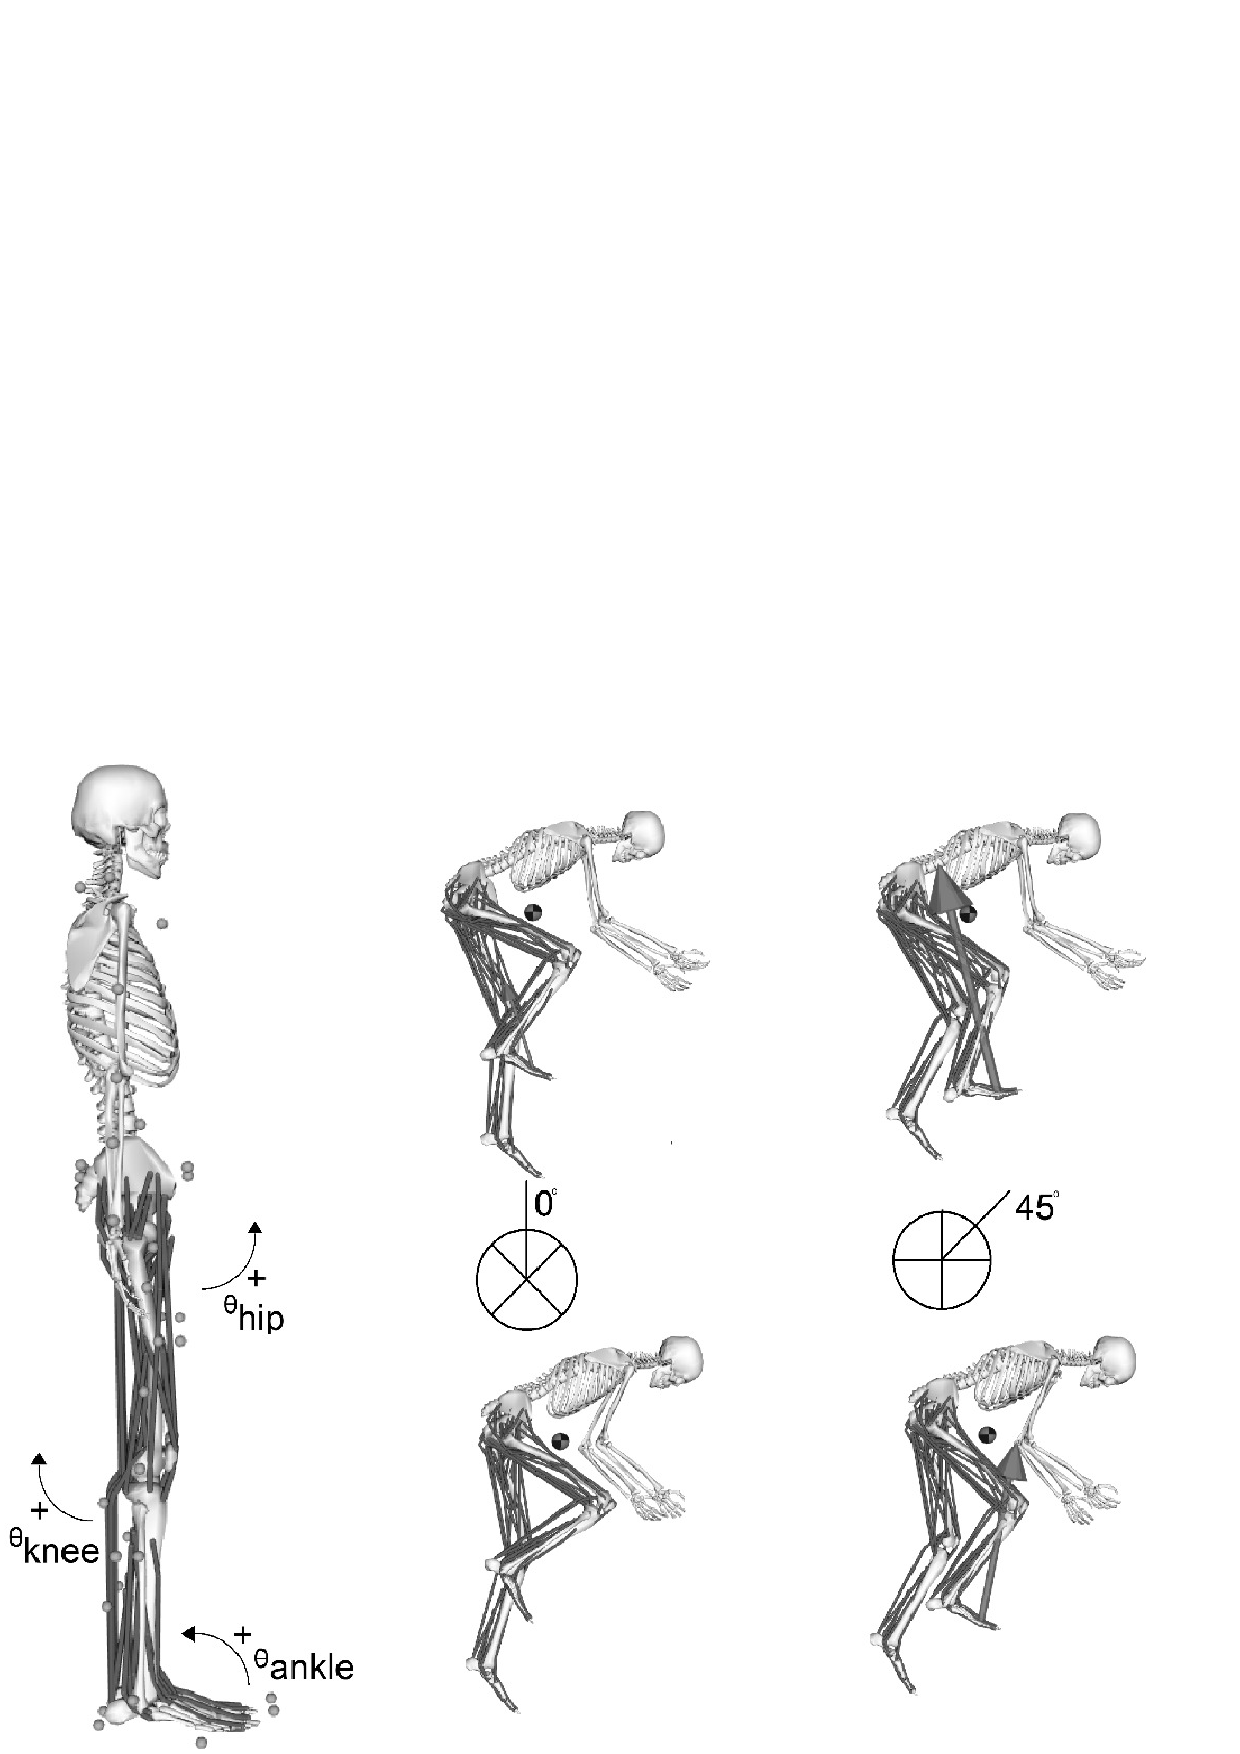
\includegraphics[width=0.7\textwidth]{Study5/Figure1.png}
    \caption[A single inertial sensor was used to estimate rider CoM displacement during non-seated cycling]{\textbf{A single inertial sensor was used to estimate rider CoM displacement during non-seated cycling.} A. An IMU attached to a rigid marker cluster was secured to the skin at the intersection of Tuffier's line (dashed) and lumbar spine midline ($\sim$L4 spinous process). B. Sagittal plane view of a scaled musculoskeletal model cycling in a non-seated posture. The kinematic estimate of the rider's CoM position is represented by the green sphere.}
    \label{fig:m4f1}
\end{figure}

\begin{table}[htbp]
    \centering
    \includegraphics[width=\textwidth]{Study5/Table1.png}
    \caption[Notation, reference coordinates, and definitions used in this study.]{\textbf{Notation, reference coordinates, and definitions used in this study.} Notation, reference coordinates, and definitions used to describe the orientation and motion of the IMU and marker cluster body in this study.}
    \label{tab:m4t1}
\end{table}

\subsection{Musculoskeletal model}
Kinematic analysis was performed using a previously developed full-body musculoskeletal model \autocite{Rajagopal2016} within OpenSim software \autocite{Delp2007}.  A static trial was collected with each participant standing in a standard-anatomical posture to scale the model to each participant's anthropometry. Segment length of the arms, trunk, and legs were scaled in all three axes using the distance between nominated marker pairs. Scaling factors were calculated by comparing these distances to that of the generic model. The mass of the participant was then used in combination with these scaling factors to distribute segment masses. The scaled model and motion capture data were used to run inverse kinematics via the Application Programming Interface between OpenSim and Matlab. The inverse kinematics tool within OpenSim calculates the position of each segment at each time step by using a weighted-least-squares fit to minimise errors between the experimental and the model markers. Segment positions as calculated by the inverse kinematic analysis are then combined with segment masses to determine the whole-body CoM location.

\subsection{Statistical analysis}
Sensor performance was quantified for each experimental condition as the root-mean-square (RMS) error in each Euler parameter describing the yaw, pitch, and roll components of the IMU angular velocity compared to the attached marker cluster body. For each trial, the mean error was calculated from the absolute error in each frame over the 10 seconds of data. The range of vertical IMU displacement within each crank cycle was compared across all experimental conditions to an attached marker cluster tracked with an optical motion capture system and to a kinematic estimate of vertical CoM displacement using a full-body musculoskeletal model. 

Agreement between the IMU and the two other measures was assessed by applying a Limits of Agreement (LoA) approach \autocite{Bland1999}. LoA analyses were corrected for repeated measures and encompassed accuracy (Bias), precision (standard deviation), average error (bias/range), and maximum error (standard deviation/range). Different LoA calculations were carried out depending on whether a significant linear trend was identified in the distribution of differences between the IMU and the two other measures (IMU \textminus measure) as a function of the mean range of vertical displacement ((IMU + measure) \textdiv 2). If a linear trend was identified, bias was calculated as the equation of the linear model, rather than a constant value \autocite{Bland2007}. Sphericity of the data was checked using Mauchly's test and non-parametric analyses were used when necessary. For non-parametric analyses, LoA were calculated as the median difference $\pm$ 1.45 times the interquartile range of differences, rather than the mean difference $\pm$ 1.96 times the standard deviation of differences. A simple linear regression was performed across all experimental conditions to identify the linear trend between the range of vertical IMU displacement to the two other measures. All statistical analyses were performed in Matlab. Normally distributed data are presented as mean $\pm$ standard deviation (SD), whereas non-normally distributed data are presented as median $\pm$ median absolute deviation (MAD). 

\begin{figure}[htbp]
    \centering
    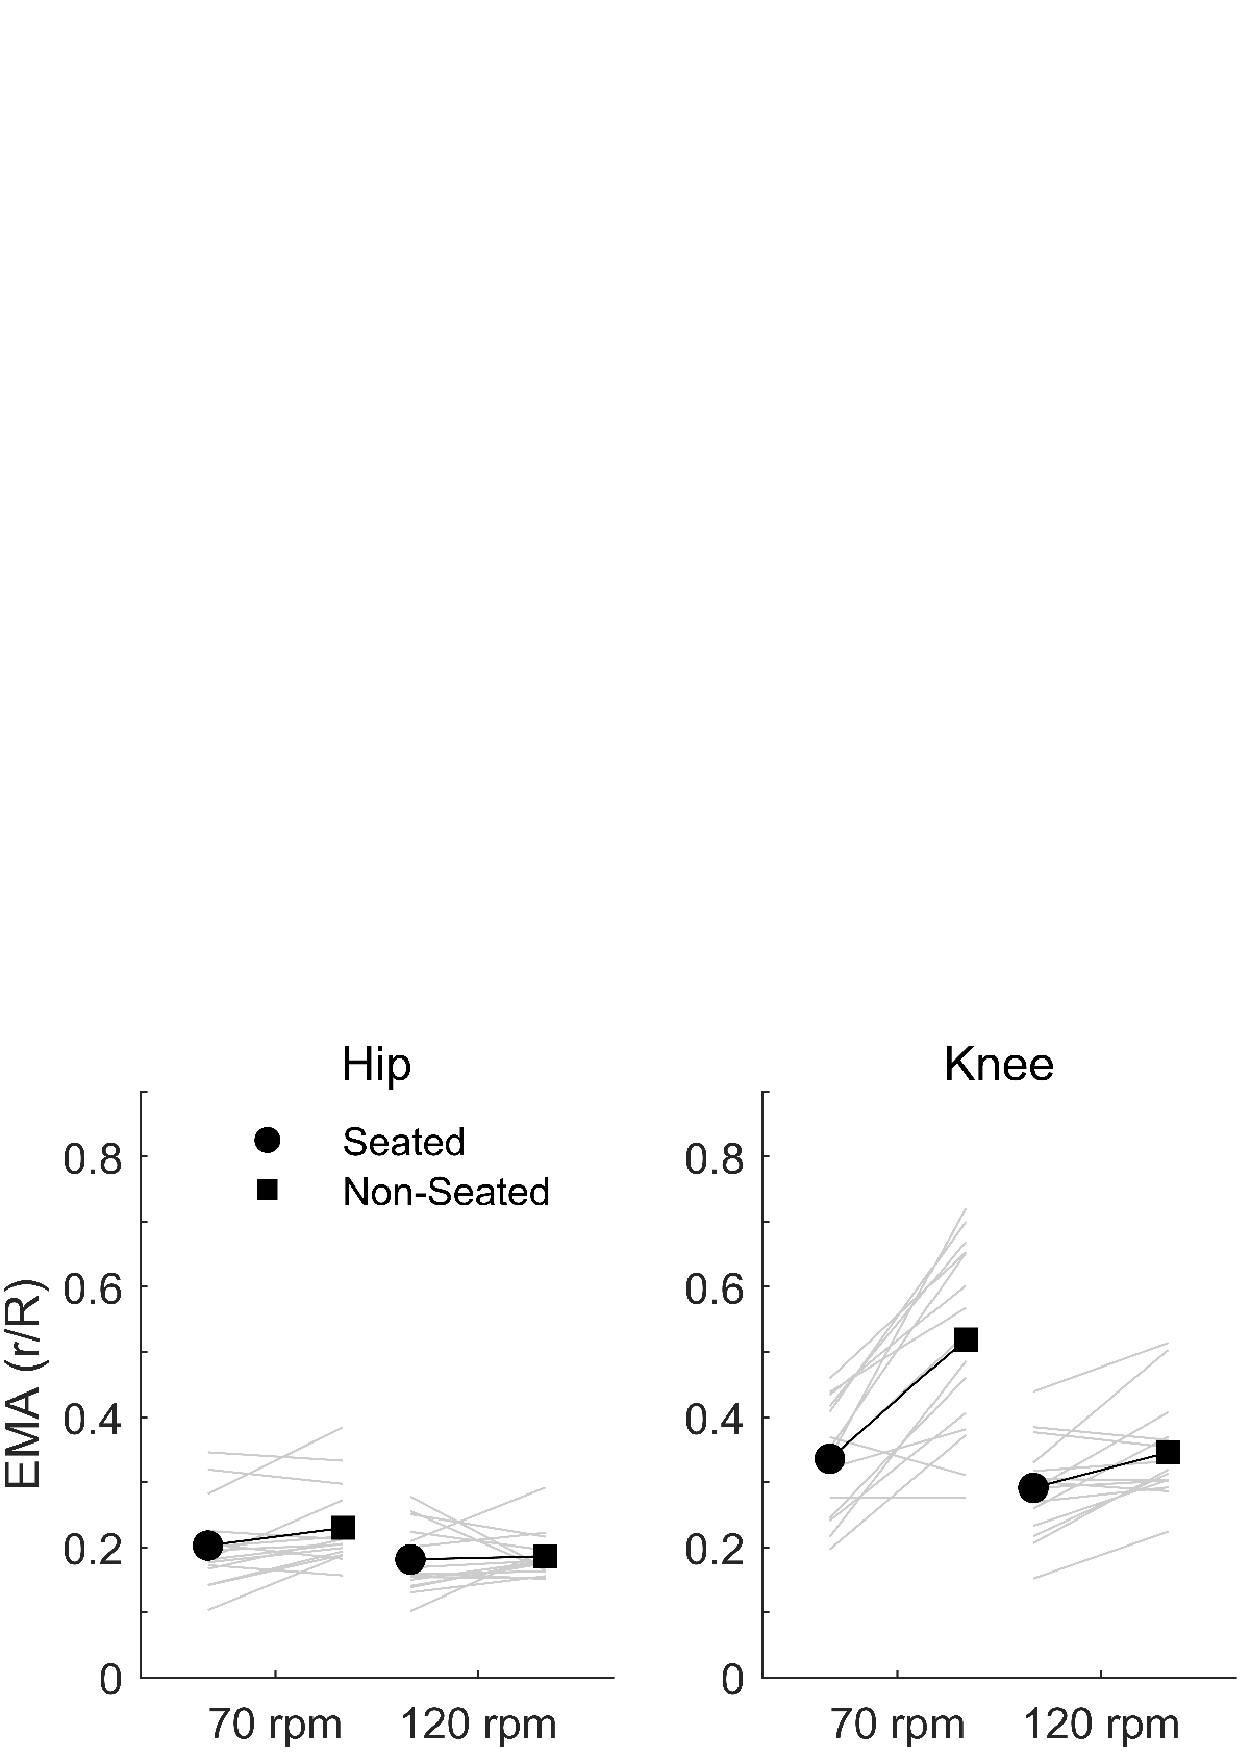
\includegraphics[width=0.6\textwidth]{Study5/Figure4.png}
    \caption[The orientation of the sensor matched nicely with the attached marker cluster]{\textbf{The orientation of the sensor matched nicely with the attached marker cluster.} Comparison of Euler angle and angular velocity parameters between the IMU and rigid marker cluster body for a single participant cycling in a non-seated posture at 30$\%$ P$_{max.i}$ at 70 rpm. All angle values are in radians and angular velocity values are in radians per second.}
    \label{fig:m4f2}
\end{figure}
\FloatBarrier

\section{Results}
To avoid any bias between the two cadence conditions at each power output, the number of cycles analysed from each participant was matched between all conditions. This meant that eight crank cycles were processed for each of the seven participants in each of the six conditions. Due to data dropout, 12 cycles were discarded, while a further 21 cycles were identified as outliers (>3 scaled median absolute deviations from the median) \autocite{Leys2013} and removed from the analysis. Thus, a total of 303 cycles were analysed ($\sim$7 cycles per condition per participant). The distribution of differences between the IMU and the two other measures violated Mauchly's test for sphericity, thus non-parametric analyses were used for all statistical comparisons.

\subsection{Sensor Performance}
The results of the sensor performance analysis are summarised in Table \ref{tab:m4t2}. Group mean ($\pm$ standard deviation) RMS errors between the IMU and marker cluster body are reported for each condition. The data shown in Figure \ref{fig:m4f2} illustrates how well the IMU was able to track the orientation and motion of the marker cluster body in all three axes.  

\subsection{IMU vs Optical motion capture}
Differences between the IMU and marker cluster's range of vertical displacement were non-normally distributed with no significant linear trend. As such, a non-parametric, constant LoA analysis was performed. Linear regression results and Bland-Altman plots are presented in Figure \ref{fig:m4f4}A and B, respectively. Across all conditions, there was high agreement between the IMU and marker cluster range of vertical displacement (See Table \ref{tab:m4t3}). On average, the IMU marginally overestimated the cluster results by 1.6 $\pm$ 3.5 mm (accuracy $\pm$ precision), which equated to an average error of 1.8 $\pm$ 3.9$\%$. Figure \ref{fig:m4f3} illustrates how well the IMU was able to track the marker cluster's vertical displacement during the crank cycle.

\subsection{IMU vs Musculoskeletal model}
Differences between the IMU and musculoskeletal model's range of vertical displacement were non-normally distributed and showed a significant linear trend. As such, a non-parametric, variable LoA analysis was performed. Linear regression results and Bland-Altman plots are presented in Figure \ref{fig:m4f4}C and D, respectively. Across all conditions, the agreement between the IMU and marker cluster range of vertical displacement decreased at higher ranges of vertical displacement (See Table \ref{tab:m4t3}). Across all conditions, the IMU substantially overestimated the cluster results, especially at higher ranges of vertical displacement. Figure \ref{fig:m4f3} illustrates the discrepancy between the IMU's vertical displacement and the model's vertical CoM displacement during the crank cycle. 

\begin{figure}[htbp]
    \centering
    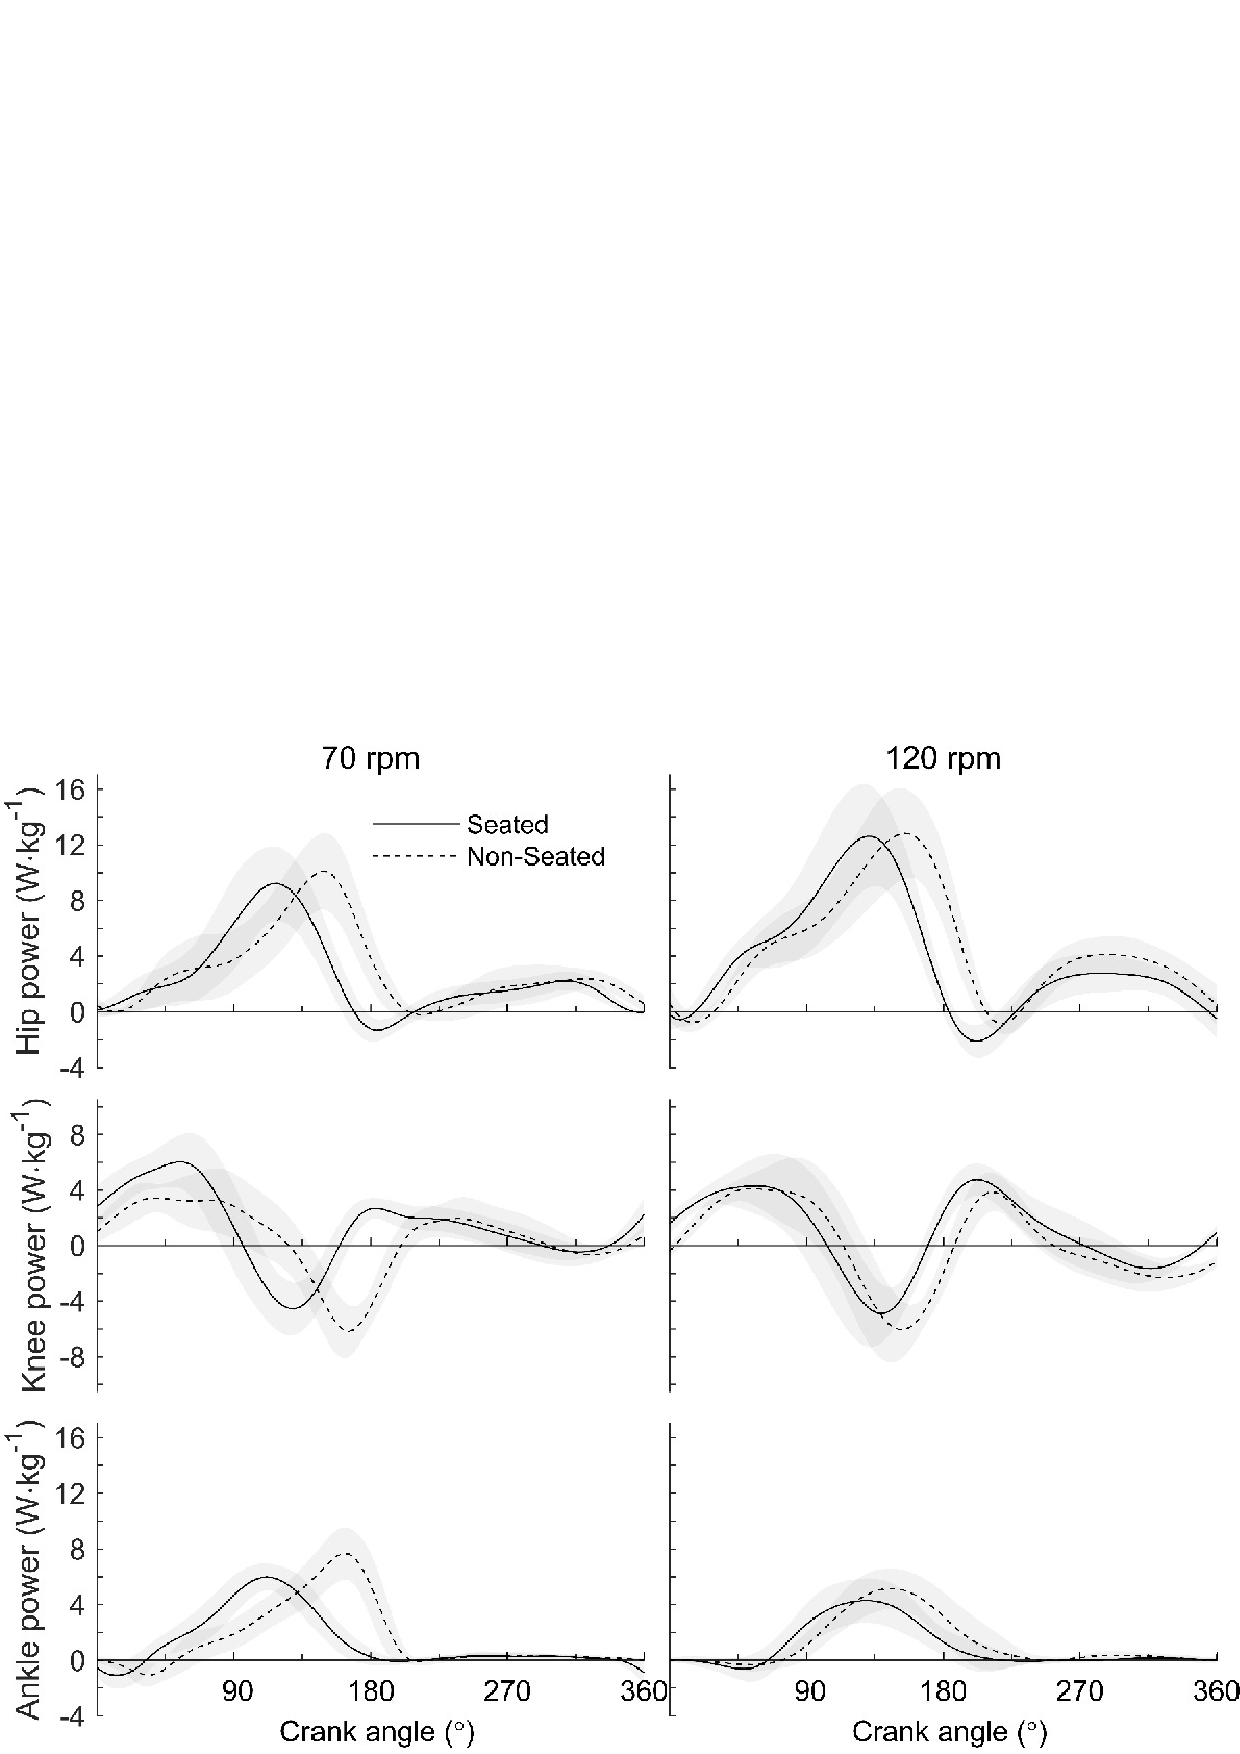
\includegraphics[width=\textwidth]{Study5/Figure2.png}
    \caption[The pattern of vertical IMU displacement matched well with the marker cluster and model's CoM]{\textbf{The pattern of vertical IMU displacement matched well with the marker cluster and model's CoM.} Group mean vertical displacement of the IMU, marker cluster body, and CoM of the musculoskeletal model with respect to crank angle (0\textdegree and 360\textdegree = top dead centre) during non-seated cycling at three power outputs (10$\%$ (A,D), 30$\%$ (B,E), and 50$\%$ (C,F) P$_{max.i}$) at 70 rpm (A-C) and 120 rpm (D-F).}
    \label{fig:m4f3}
\end{figure}

\begin{table}[htbp]
    \centering
    \includegraphics[width=\textwidth]{Study5/Table2.png}
    \caption[The sensor performance was excellent across all conditions] {\textbf{The sensor performance was excellent across all conditions.} Group mean ($\pm$ standard deviation) RMS error in each Euler parameter describing the yaw, pitch, and roll components of the IMU angular velocity (rad$\cdot$s$^{-1}$) compared to the rigid marker cluster body during non-seated cycling at three different power outputs (10$\%$, 30$\%$, and 50$\%$ P$_{max.i}$) and two different cadences (70 rpm and 120 rpm).}
    \label{tab:m4t2}
\end{table}

\begin{figure}[htbp]
    \centering
    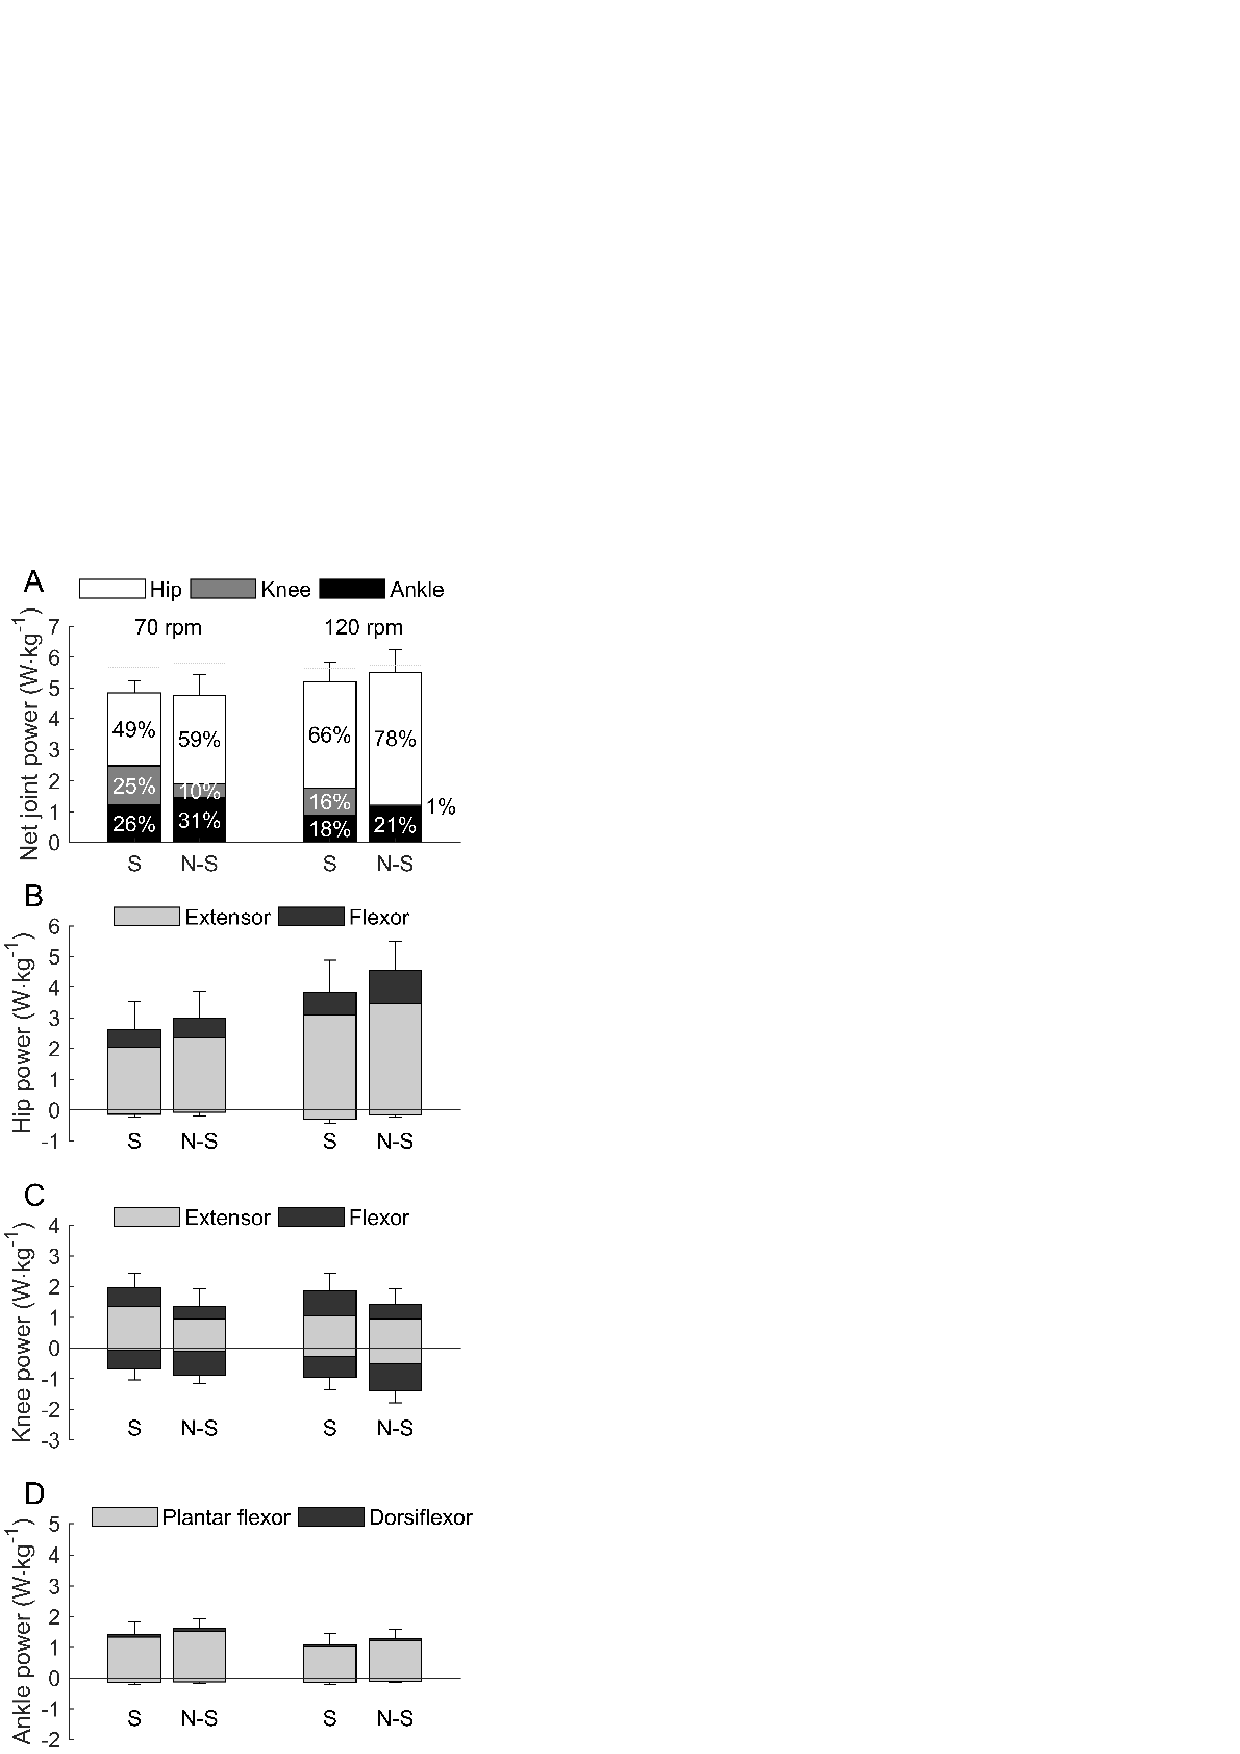
\includegraphics[width=\textwidth]{Study5/Figure3.png}
    \caption[The IMU tracked the cluster with high accuracy, but overestimated the model's range of vertical CoM displacement]{\textbf{The IMU tracked the cluster with high accuracy, but overestimated the model's range of vertical CoM displacement.} A. Regression (left) and Bland-Altman plots (right) of the range IMU vertical displacement within each crank cycle as a function of Cluster vertical displacement (top) and Model CoM vertical displacement (bottom). The non-parametric repeatability coefficient (RPC$_{np}$) is also shown as a percentage of mean displacement.}
    \label{fig:m4f4}
\end{figure}

\begin{table}[htbp]
    \centering
    \includegraphics[width=\textwidth]{Study5/Table3.png}
    \caption[There was good agreement between the IMU and cluster, but not between the IMU and model] {\textbf{There was good agreement between the IMU and cluster, but not between the IMU and model.} A fixed limits of agreement analysis was used to compare the range of vertical displacement derived from an IMU to a rigid marker cluster. Positive values indicate an overestimation of the marker cluster's vertical displacement by the IMU (IMU \textminus Cluster). All measures are in millimetres. A variable limits of agreement analysis was used to compare the range of vertical displacement derived from an IMU to the musculoskeletal model. All measures are in millimetres.}
    \label{tab:m4t3}
\end{table}

\FloatBarrier

\section{Discussion}
The present study aimed to assess the suitability of a single IMU for tracking the vertical displacement of a rider's CoM displacement during non-seated cycling at three power outputs and two cadences. We found that the IMU overestimated the kinematic estimate of vertical CoM displacement and that this overestimation increased linearly with respect to the measured range of vertical CoM displacement. The IMU was able to identify the trend that the range of a rider's vertical CoM displacement during non-seated cycling increases in response to increasing power output and time per crank cycle, however, it underestimated the rate of this increase. The lowest power output trial in this study was approximately 2.1 W$\cdot$kg$^{-1}$, which is typical of steady-state cycling in a seated posture, suggesting that the IMU is likely to be more accurate during steady-state conditions compared to very-high-power output conditions. However, it should be noted that the non-seated posture is typically used for producing high-power outputs during climbing and sprinting. 

We interpret our findings as evidence that a single IMU can track the vertical displacement of an attached marker cluster with high accuracy and precision, but unacceptable discrepancies exist between the vertical displacement of the IMU and the kinematic estimate of rider CoM displacement. While discrepancies between the single IMU and rider CoM increased with increasing power output and decreasing cadence, these increases were systematic and may be able to be accounted for using linear regression.

Across all trials, the IMU tracked the attached marker cluster with high accuracy and precision, but substantially overestimated the kinematic estimate of rider CoM displacement. This suggests that a rider's lower back goes through a larger range of vertical displacement during each crank cycle than their CoM. This makes intuitive sense as the motion of body segments other than the torso have a significant influence on the whole-body CoM. For example, previous research on seated cycling shows that the total segmental energy of the legs fluctuates during each crank cycle, predominantly due to changes in potential energy \autocite{Kautz2002}. However, just as the range of CoM displacement increased in response to increasing power output, so too did the absolute difference between lower back and CoM displacement. This suggests that negative work done by the arms \autocite{Turpin2016,Wilkinson2020b} likely acts on the torso to decouple lower back movement from the torso CoM. Thus, it is evident that a single IMU on the lower back cannot account for the entirety of changes in CoM position due to motion of the legs and rotation of the torso during non-seated cycling.

We cannot rule out that a portion of the disagreement between the IMU and model was due to the processing of the IMU data, however, the accuracy between the IMU and cluster suggests the portion of disagreement due to processing errors was minimal. It is possible that small offsets were present due to the manual synchronisation process between the IMU and motion capture data, which could be avoided in future studies by using hardware-synchronised systems. Another possible source of error was the misalignment between the IMU and marker cluster. The IMU was attached using a silicone putty which prevented any relative movement but does not guarantee that the alignment to the plane created by the marker clusters was exact. A misalignment between the IMU and marker cluster would cause a constant offset in the orientation data, however, small errors in orientation are known to have a minimal influence on linear displacements in a global-coordinate system (Pfau, Witte, and Wilson 2005). 

Our data suggest that a single IMU placed on the lower back is not sufficient for tracking a rider's CoM displacement during non-seated cycling. It is possible that multiple IMUs would provide a solution to this problem, however, any additional weight or restriction of movement due to such a system would likely prevent its widespread use during cycling. It is possible that another location on the body may provide superior tracking of the CoM compared to the lower back. In general, the location of the CoM during non-seated cycling is in front of the pelvis and outside the body (See Figure \ref{fig:m4f1}). Thus, an IMU placed on the front of the pelvis would be closer to the CoM, however, this location would still be unable to account for the influence of leg motion on CoM movement. Furthermore, we suspect that this location may be more likely to suffer from greater soft-tissue movement not related to the CoM movement \autocite{Riddick2016}. 

A single IMU placed on the lower back may still be suitable for other applications in the analysis of cycling. For example, a single IMU is lightweight and relatively low-cost, meaning it could provide a low-cost solution for identifying when a cyclist changes their posture from seated to non-seated. Our data suggest that the precision of the IMU would be adequate for providing within-condition comparisons. Our findings are in agreement with previous research that IMUs provide an accurate and precise measure of orientation and displacement of attached objects. Thus, a single IMU attached to the frame of a bicycle would be suitable for measuring the angular displacement and velocity of the bicycle frame; this and many other analytics could be provided by integrating an IMU with a cycling computer. 

In summary, we found that, during non-seated cycling, a single IMU placed on the lower back overestimates a rider's vertical CoM displacement: as this displacement increases, the overestimation error increases linearly. Further development of a single-IMU method for measuring a rider's CoM displacement and associated mechanical energy fluctuations during over-ground cycling remains a future goal.
